Since blockchain technology is proposed, different methods are experimented for visualization. As Bitcoin is the first and main blockchain network in the world and the data can be accessed publicly, much literature uses it as a research platform. Generally, there are three categories of related works for the visualization of a blockchain system.
\begin{itemize}
    \item \textbf{Visualization of Blockchains} \\
        There are a lot of online visualization tools which can visualize the static information of transactions and blocks on a blockchain system. They display the information in detail and provide it as the base for analysis.
    \item \textbf{Analysis of Transactions} \\
        As Bitcoin becomes a popular peer-to-peer network recently, most of the recent literature focuses on the analysis of the relationships between transactions and blocks in Bitcoin network. They try to recognize special patterns to gain ecnomic experience and prevent criminal activities.
    \item \textbf{Analysis of Consensus Protocols} \\
        An analysis of the consensus protocols on the blockchain networks is an interesting topic as it can reveal the potential applications on blockchain platforms.
\end{itemize}

\section{Visualization of Blockchains}

There are some online tools and applications that provide visualization of the static status of transactions and blocks in Bitcoin. Tri A. Sundara et al. \cite{Sundara2017} summarized 8 visualization applications and compared their visualization methods and technologies. We shortly reivew these applications here, so the main difference of our application and them can be identified clearly.

Bitbonkers \cite{bitbonkers} rendered a live 3D animation of transactions and blocks. Balls represented transactions, and they kept dropping down to the plate from the top. On the other hand, cubics represented blocks. The sizes of balls are different according to their values. Bitnodes \cite{bitnodes} focused on the visualization of the distribution of nodes on Bitcoin network. BitcoinCity \cite{bitcoincity} was a cute visualization of Bitcoin. It used a road to chain the blocks, and the houses with different heights on the both sides of the road represented transactions. Blockseer \cite{blockseer} visualized the detailed information of accounts, transactions or blocks with tree structures. DailyBlockchain \cite{dailyblockchain} displayed the spread of dynamic and live Bitcoin network. Elliptic \cite{elliptic} visualized the whole history of Bitcoin like the Big Bang of the universe. Interaqt \cite{interaqt} rendered the Bitcoin transactions as circles. Live Globe \cite{liveglobe} combined the geographies of blocks and the earth together in the visualization. The screenshots of the above works are in Figure \ref{fig:visualization of bitcoin}.

\begin{figure}[htb]
    \centering
    \begin{subfigure}[b]{0.3\textwidth}
        \centering
        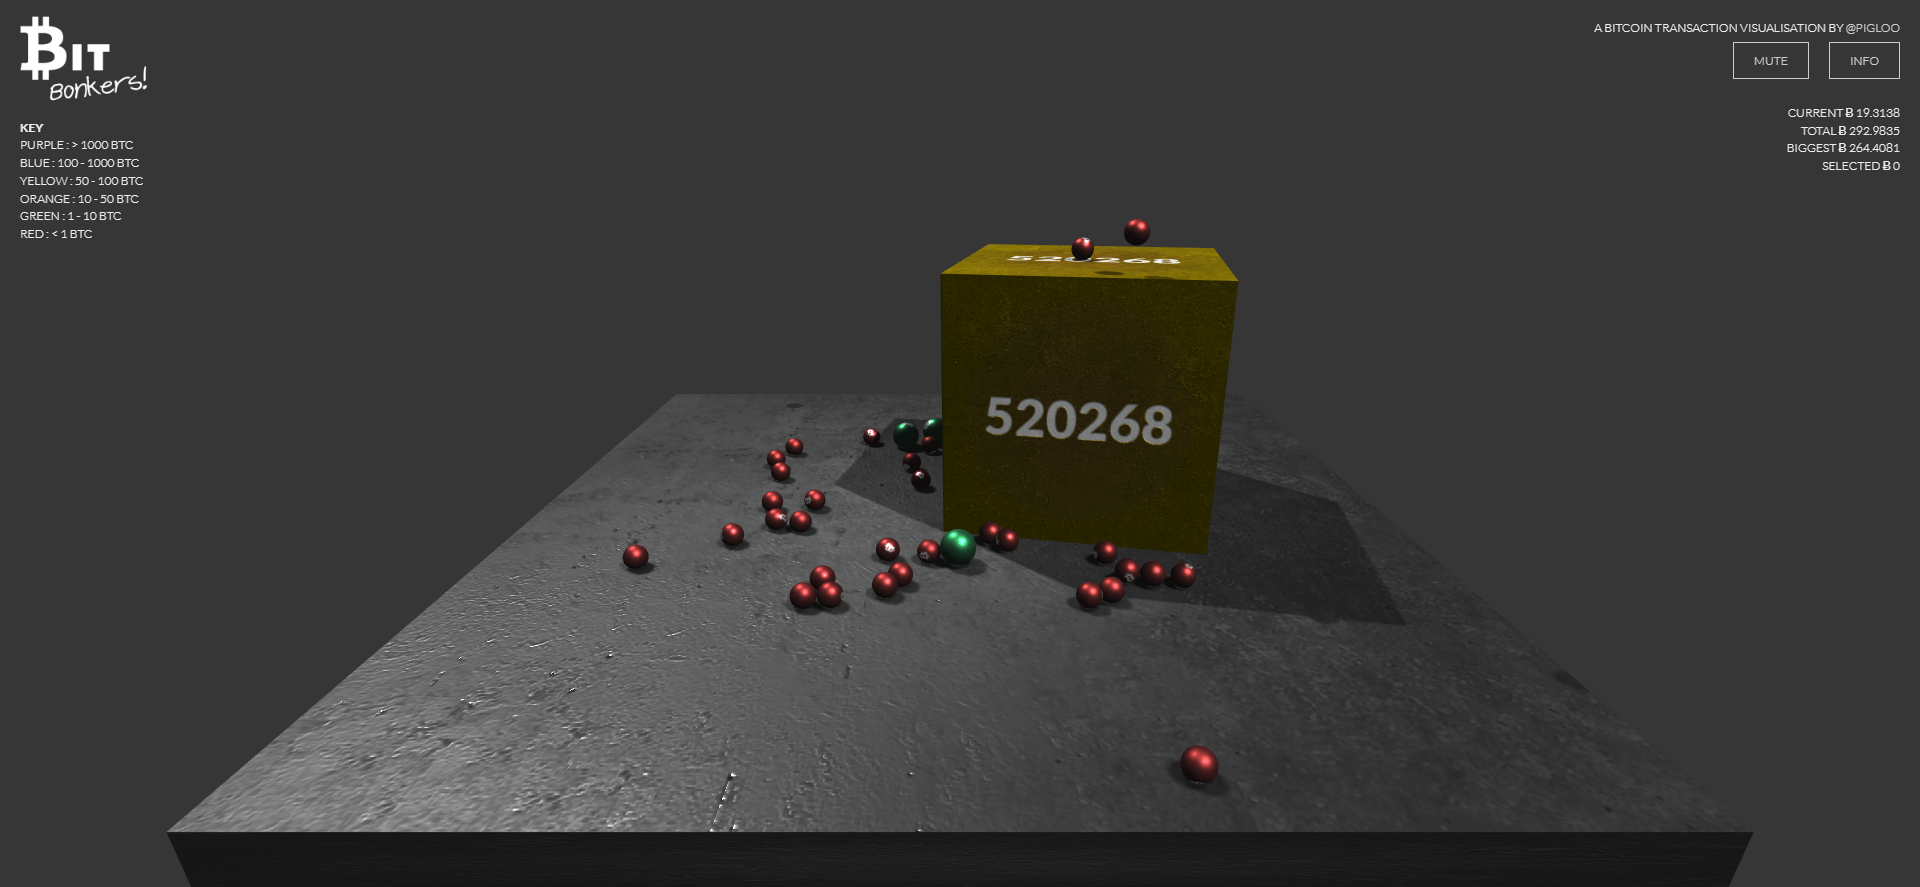
\includegraphics[width=\textwidth]{related_bitbonkers}
        \caption{Bitbonkers}
    \end{subfigure}
    \hfill
    \begin{subfigure}[b]{0.3\textwidth}
        \centering
        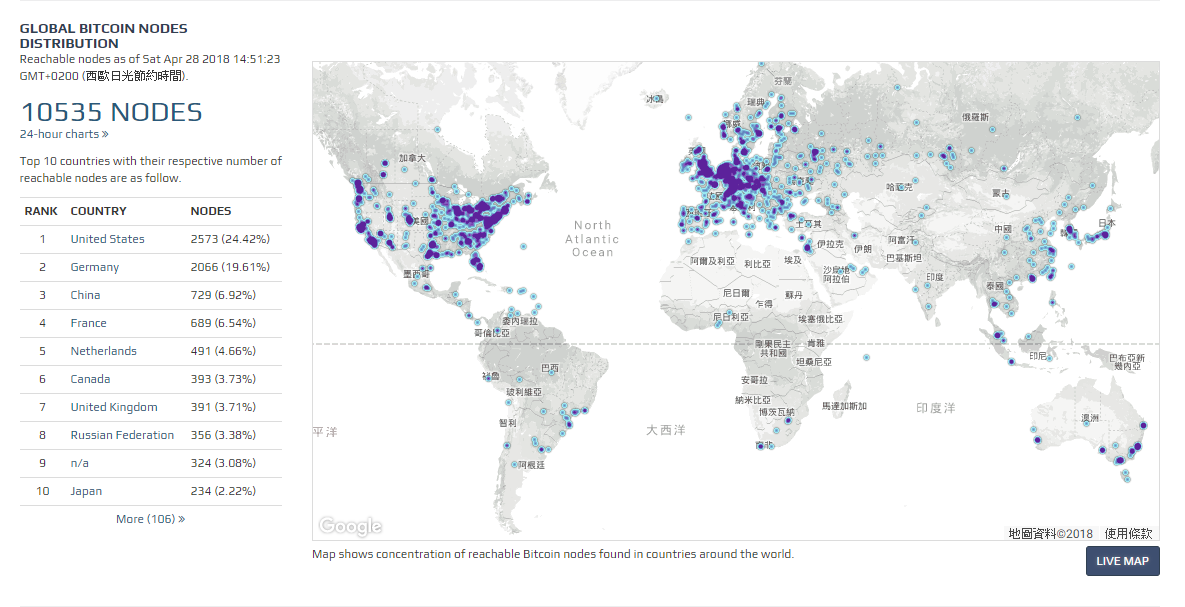
\includegraphics[width=\textwidth]{related_bitnodes}
        \caption{Bitnodes}
    \end{subfigure}
    \hfill
    \begin{subfigure}[b]{0.3\textwidth}
        \centering
        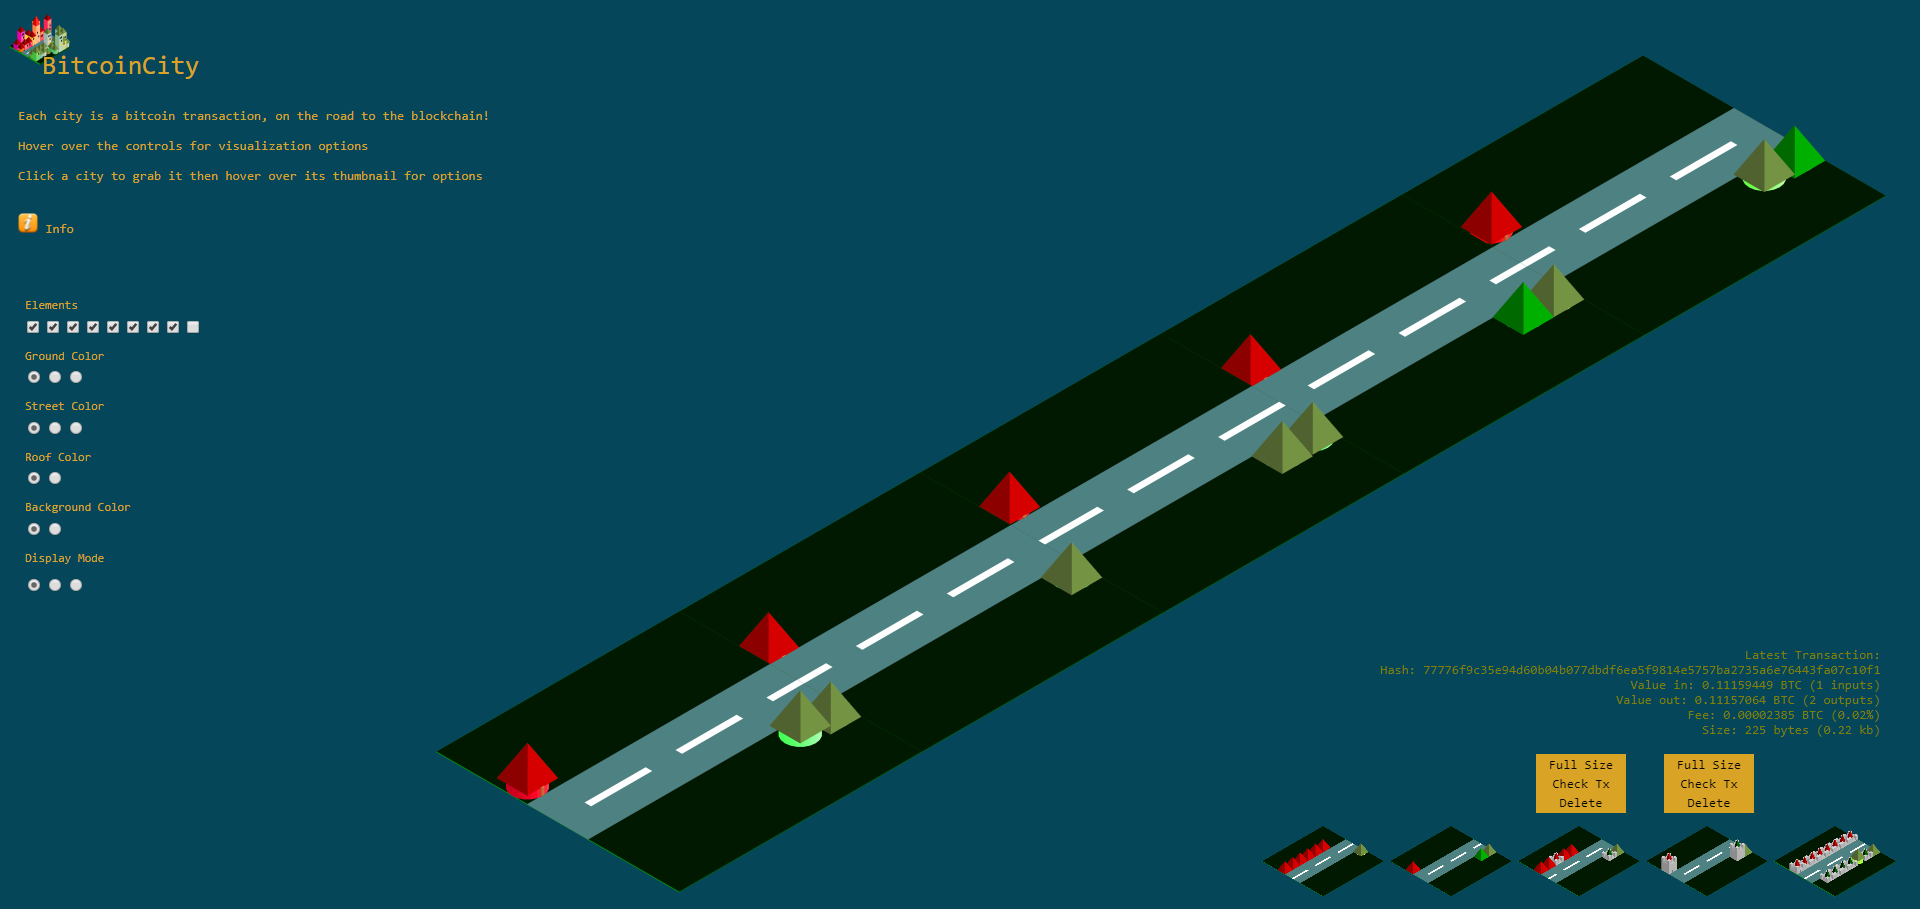
\includegraphics[width=\textwidth]{related_bitcoincity}
        \caption{BitcoinCity}
    \end{subfigure}

    \begin{subfigure}[b]{0.3\textwidth}
        \centering
        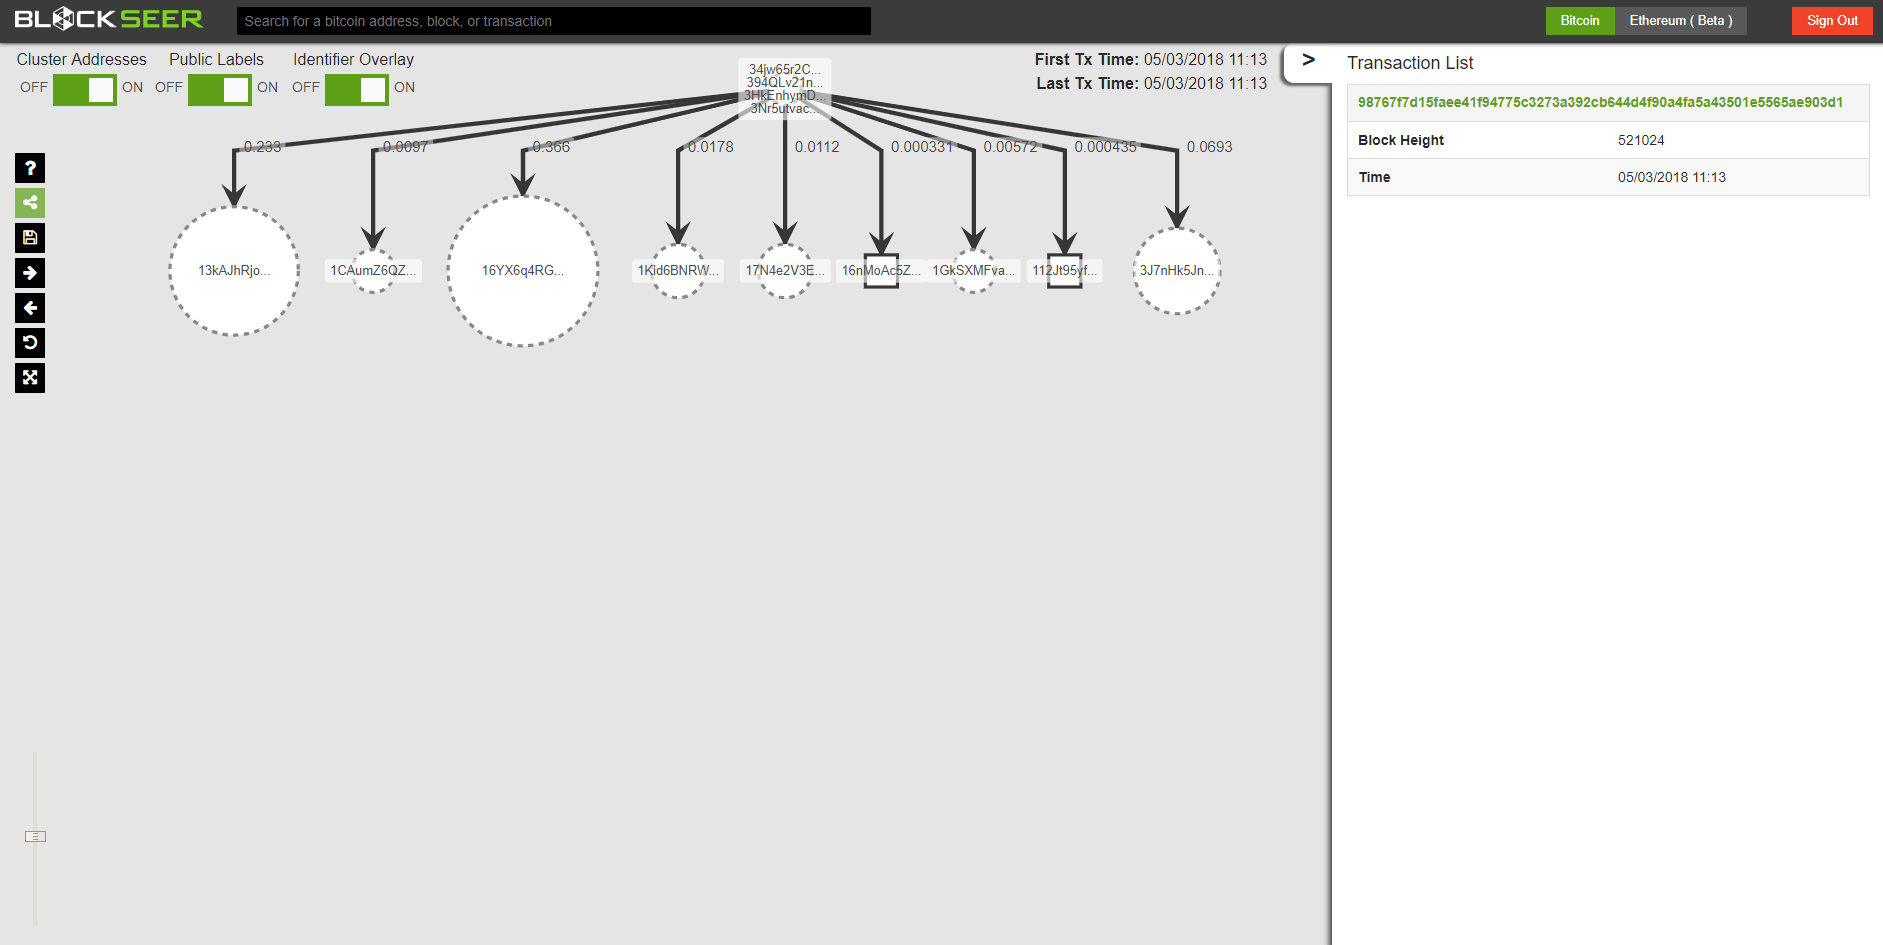
\includegraphics[width=\textwidth]{related_blockseer}
        \caption{Blockseer}
    \end{subfigure}
    \hfill
    \begin{subfigure}[b]{0.3\textwidth}
        \centering
        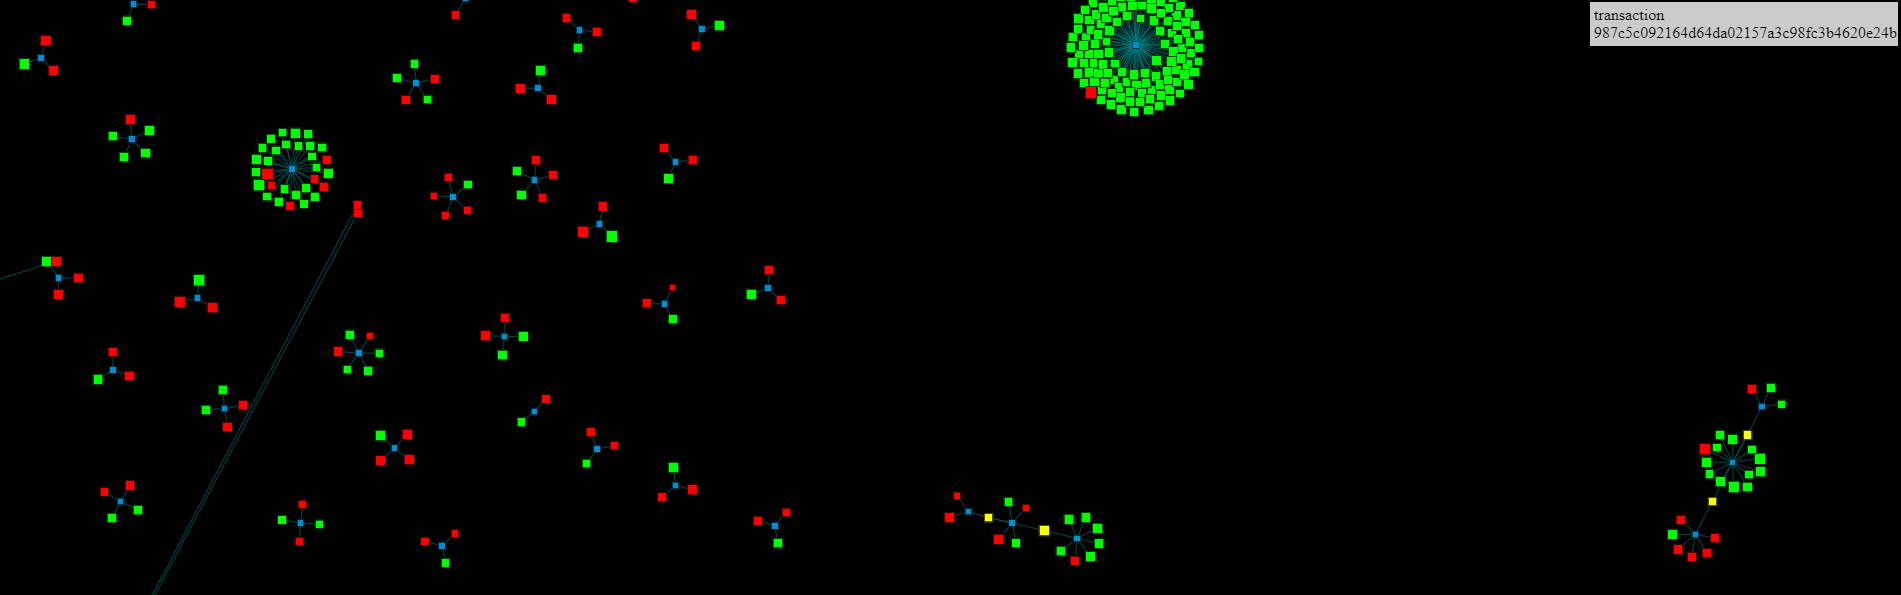
\includegraphics[width=\textwidth]{related_dailyblockchain}
        \caption{DailyBlockchain}
    \end{subfigure}
    \hfill
    \begin{subfigure}[b]{0.3\textwidth}
        \centering
        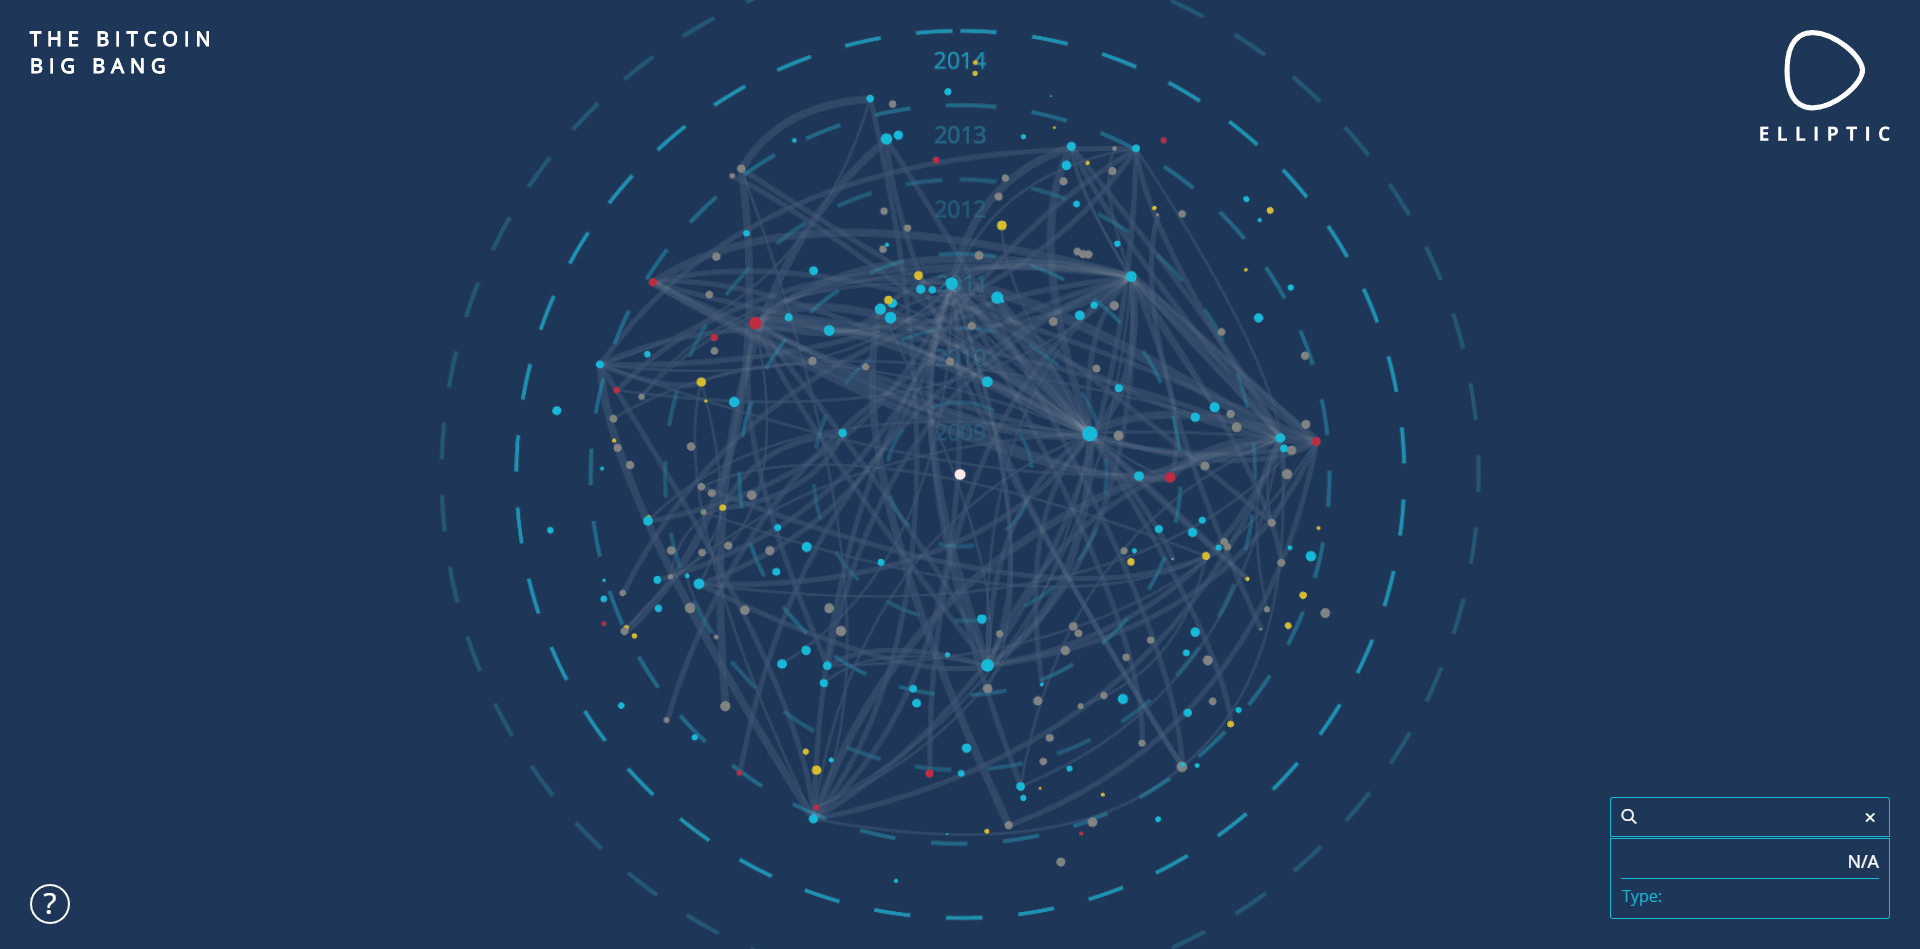
\includegraphics[width=\textwidth]{related_elliptic}
        \caption{Elliptic}
    \end{subfigure}

    \begin{subfigure}[b]{0.3\textwidth}
        \centering
        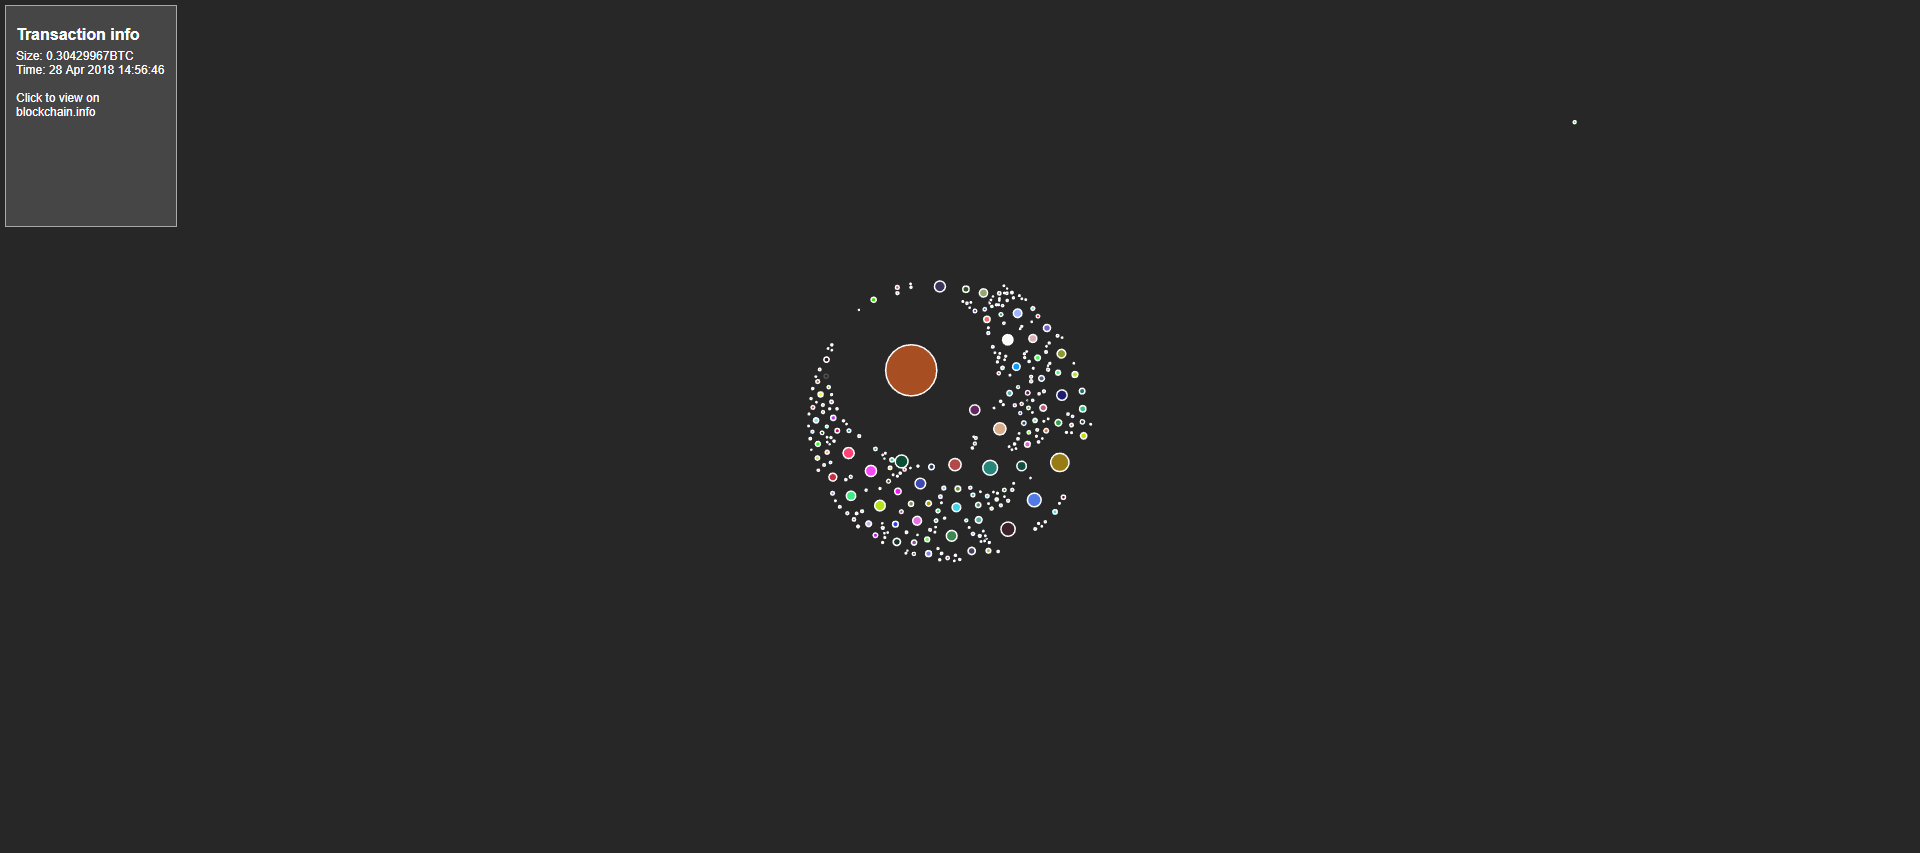
\includegraphics[width=\textwidth]{related_interaqt}
        \caption{Interaqt}
    \end{subfigure}
    \hspace{1cm}
    \begin{subfigure}[b]{0.3\textwidth}
        \centering
        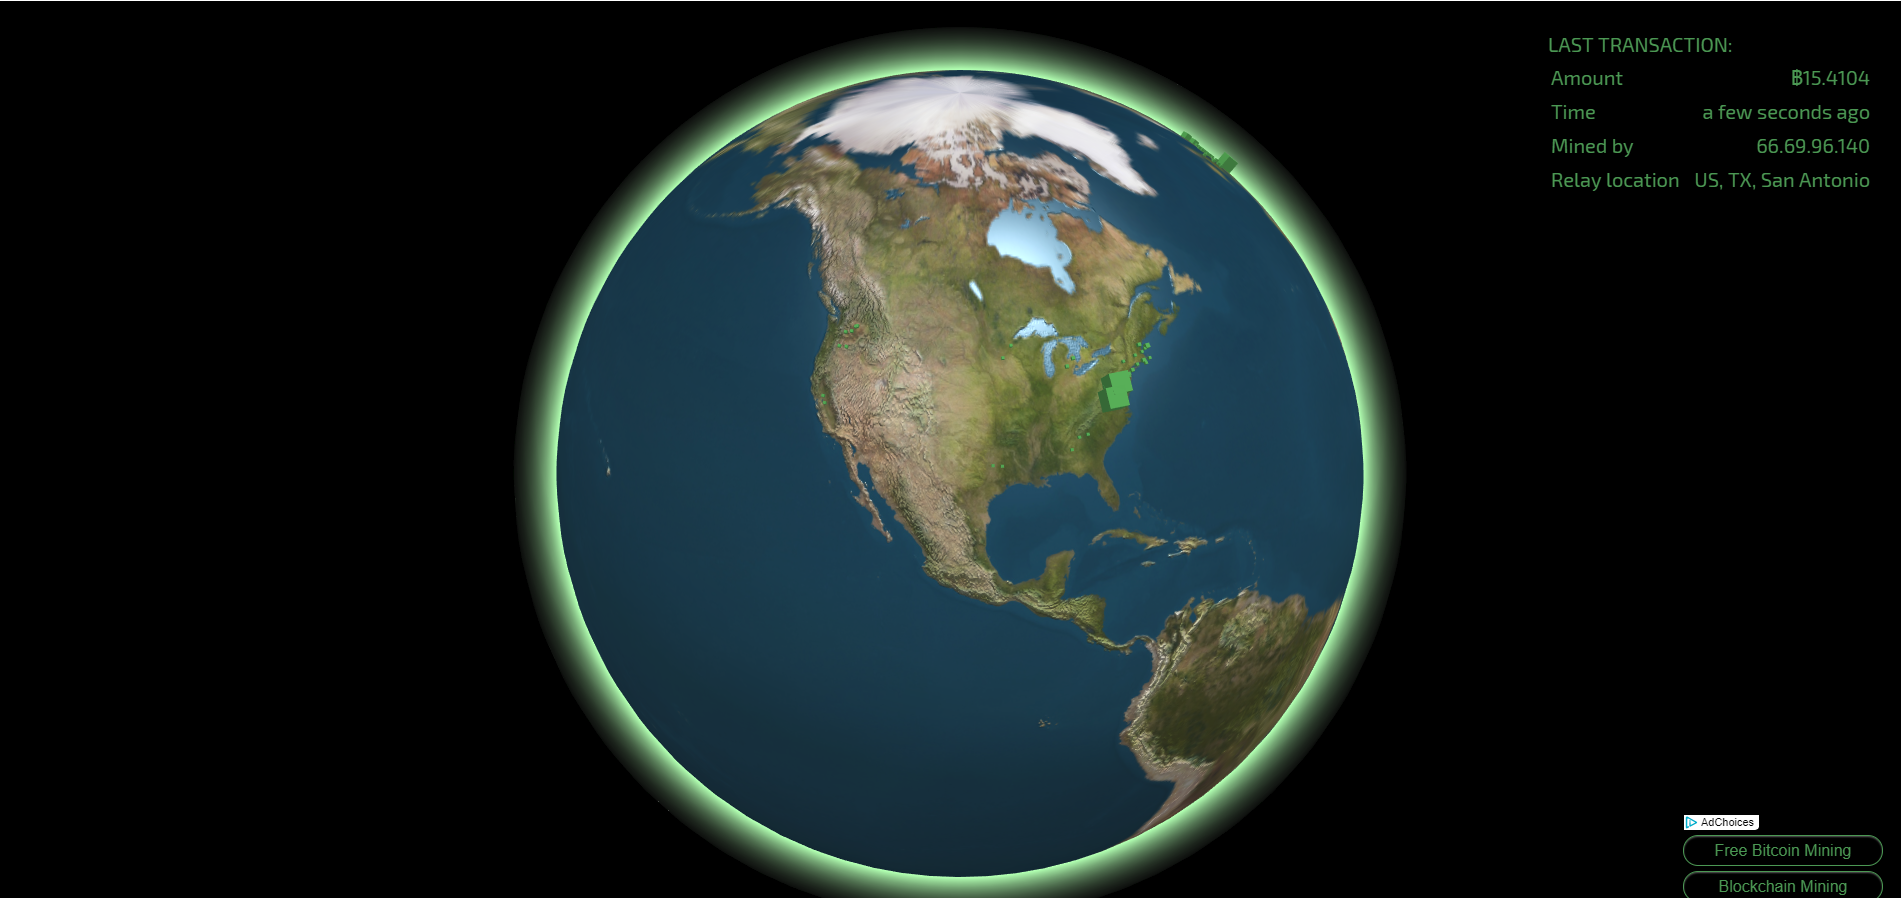
\includegraphics[width=\textwidth]{related_liveglobe}
        \caption{Live Globe}
    \end{subfigure}

    \caption{Visualization of Bitcoin}
    \label{fig:visualization of bitcoin}
\end{figure}

In addition to the 2D and 3D animations of the visualization of Bitcoin, there are applications which use tabular methods as the presentation of blockchains. Blockchain \cite{blockchain} and Etherscan \cite{etherscan} displayed the information of transactions and blocks in detail on Bitcoin and Ethereum networks. The results of them are demonstrated in Figure \ref{fig:tabular visualization}.

\begin{figure}[htb]
    \centering
    \begin{subfigure}[b]{0.4\textwidth}
        \centering
        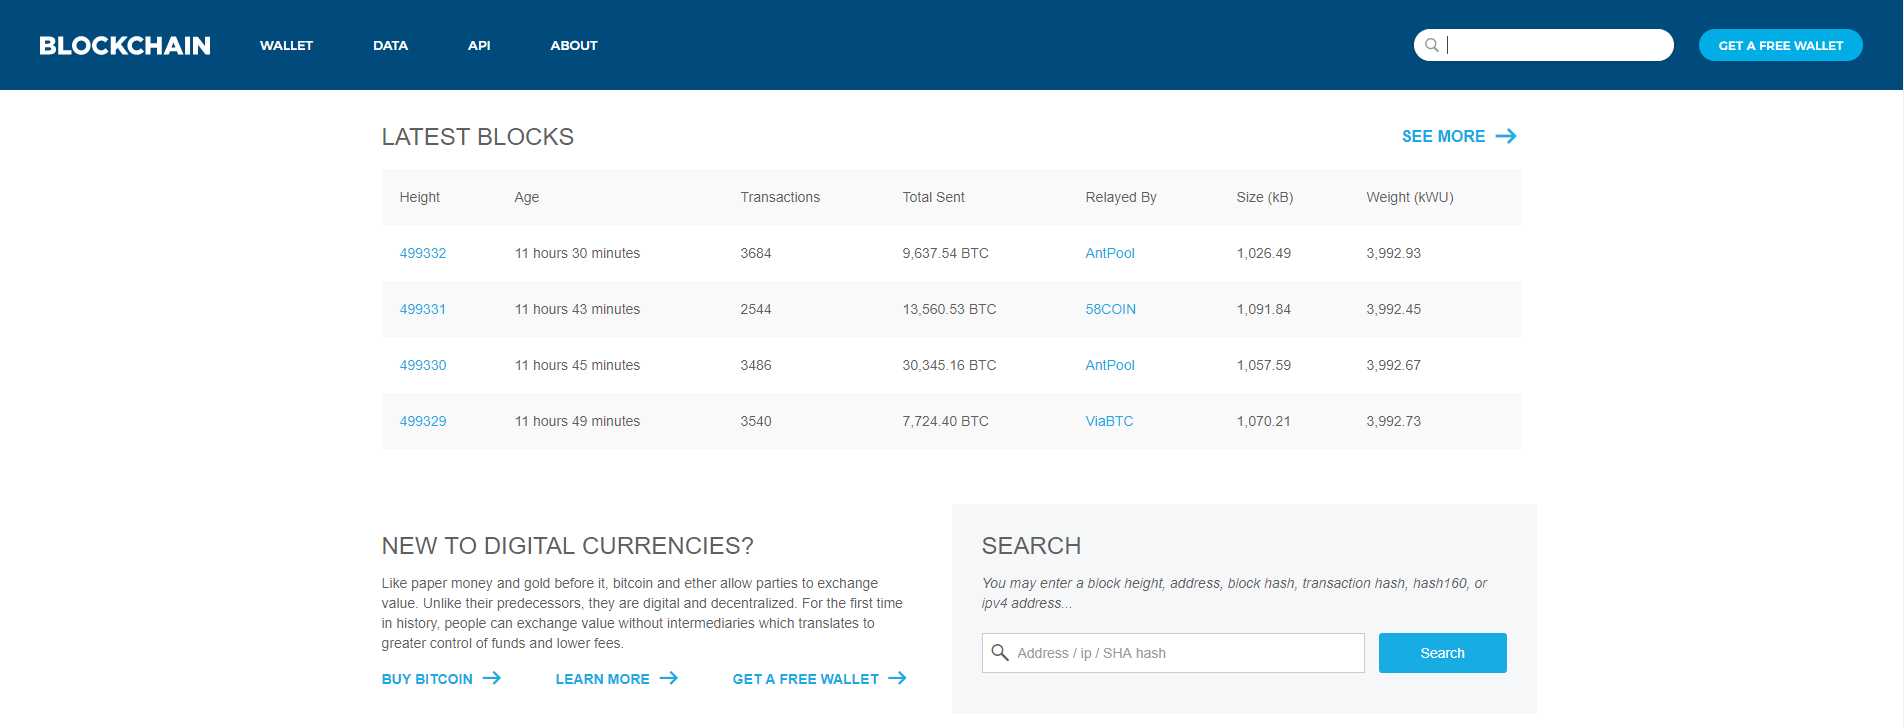
\includegraphics[width=\textwidth]{related_blockchain}
        \caption{Blockchain}
    \end{subfigure}
    \hfill
    \begin{subfigure}[b]{0.4\textwidth}
        \centering
        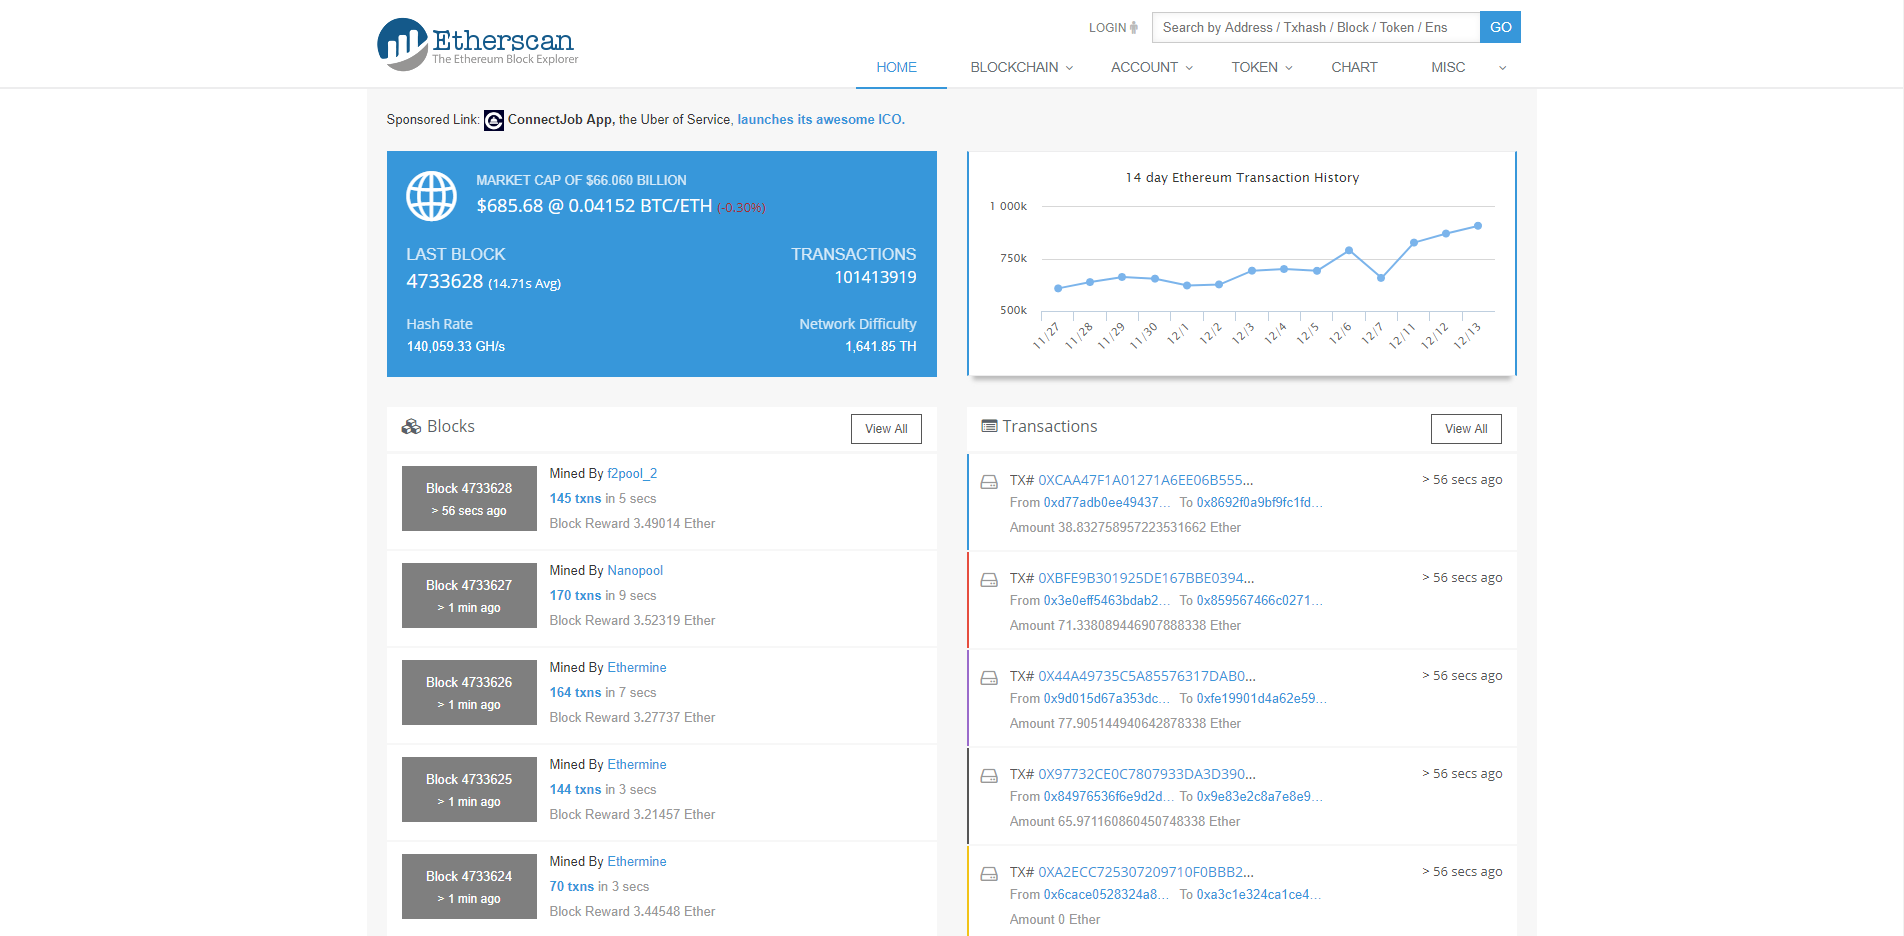
\includegraphics[width=\textwidth]{related_etherscan}
        \caption{Etherscan}
    \end{subfigure}

    \caption{Tabular Visualization}
    \label{fig:tabular visualization}
\end{figure}

In short conclusion, although the above tools and applications showed amazing visualization methods of blockchains, their goals were to provide the static information and statistics instead of the dynamic mining processes that happened in a blockchain system. It is difficult to gain valuable understandings about the complex and dynamic mining processes in these applications.

\section{Analysis of Transactions}

Most of the visualization tools of Bitcoin are focused on the analysis of the relationships between transactions in time series. Giuseppe Di Battista et al. \cite{Battista2015} provided a visualization tool called BitConeView that analyzed the flows of bitcoins in the transactions by timestamps. It can be used to analyze the patterns of the flows of bitcoins and locate tainted transactions. To prevent the criminal activities and illegal behaviors that abuse the services of Bitcoin, Hiroki Kuzuno et al. \cite{Kuzuno2017} proposed an analyzing system which managed the data and statistics of blockchains for the usages of law enforcement investigation and training. Dan McGinn et al. \cite{McGinn2016} focused on visualizing transactions of Bitcoin from the top-down viewpoint. The visualization of the large scale of data provided domain experts and the general public a tool to analyze and identify the transaction patterns with big data visualization methods. The visual analytics tool that was proposed by Loïs Saublet \cite{Saublet2015} enabled economists to analyze the metrics and actors in Bitcoin and provided good user experience by working together with end users.

In short conclusion, the goals of the above tools and applications were to analyze the patterns and relationships of transactions and blocks. Thus, they tended to provide the static information and statistics instead of the dynamic mining processes that happen in a blockchain system. To focus on the dynamic mining activities, our tool provides a clear, real-time visualization of mining processes that cannot be achieved by the above analysis tools.


\section{Analysis of Consensus Protocols}

To analyze the network conditions of the proof-of-work based blockchain system, Amitai Porat et al. \cite{Porat} provided an application that was based on Ethereum platform. It simulated the asynchronous mining activities and network latency and provided a real-time analysis of the blockchain system.

The main difference to our work is that we assume that miners have individual mining strategies instead of solving the same puzzles asynchronously. Therefore, there are miners who are able to solve the puzzles faster than the others under the same computing power, but they may suffer lower mining rewards. The combination of different mining strategies and delays of networks makes the visualization of the blockchain system dynamic and interesting, and it is suitable for researchers to find the influences of them on the blockchain system.

\section{Our approach}

To focus on the dynamic mining activities, our tool provides a clear, real-time visualization of mining processes that cannot be achieved by the above analysis tools.

There is a former project called “Kooperative Music Box” \cite{musicbox}, which was developed by Fraunhofer Blockchain-Labor. It used shapes and colors to distinguish different blocks and transactions which were generated by different nodes. The basic visualization ideas of our project are inspired by this application.

Our project aims to visualize all the dynamic mining processes that could happen in a blockchain system, with the factors of the different mining strategies and the delays of networks. This distinguishes our project to all the projects mentioned before. Therefore, our project is worthwhile as a contribution and trial to the blockchain research area.
